% =======================================================
% 5. SCRITTURA E FORMATTAZIONE
% =======================================================
\subsection{Scrittura e Formattazione Markdown}
Sotto la barra in cui compaiono le modalità di visualizzazione e di gestione dei file si trova la barra con le funzionalità centrali dell'editor divise in cinque categorie.

\subsubsection{Stile}
La prima parte è denominata "Stile" ed è composta da 6 bottoni, che da sinistra a destra sono:
\begin{enumerate}
    \item Grassetto,
    \item Corsivo,
    \item Sottolineato,
    \item Barrato,
    \item Citazione,
    \item Intestazione,
\end{enumerate}

i quali, quando vengono premuti, applicano lo stile corrispondente al blocco di testo selezionato, 
mentre nel caso non sia selezionato del testo lo stile viene applicato sul testo che verrà successivamente scritto.

Se i bottoni vengono cliccati quando il testo selezionato presenta già lo stile scelto (ad 
esempio, premo "G" (grassetto) mentre è selezionato del testo già in grassetto (\texttt{**testo**})) lo stile verrà rimosso.

\subsubsection{Elenchi}
La seconda parte è denominata "Elenchi" ed è composta da 4 bottoni, i quali da sinistra a destra sono:
\begin{enumerate}
    \item Elenco puntato,
    \item Elenco numerato,
    \item Aumenta rientro,
    \item Riduci rientro,
\end{enumerate}

\paragraph{Elenco puntato e numerato} Se applicati ad una porzione di testo non ancora organizzata in elenco, creano un elenco del tipo scelto (puntato 
o numerato); se applicati a un elenco già dello stesso tipo, rimuovono la formattazione, riportando il testo al formato normale; se applicati 
a un elenco esistente ma di tipo diverso, lo convertono al tipo appena selezionato (ad esempio, da puntato a numerato), invece di rimuoverlo. 

Se è presente una selezione di testo, l'operazione viene applicata al
blocco selezionato; in assenza di selezione, viene applicata al testo che verrà scritto
successivamente.

\paragraph{Aumenta e riduci rientro} A differenza dei due bottoni precedenti, questi due comandi non hanno un comportamento di tipo toggle: ogni click 
di "Aumenta rientro" aggiunge un ulteriore livello di rientro all'elemento selezionato, permettendo di creare elenchi annidati 
su più livelli tramite pressioni successive; ogni click di "Riduci rientro" riduce il rientro di un livello, fino a riportarlo 
a zero. Nessuno dei due rimuove l'elenco in sé.

\subsubsection{Link e Tabelle}
La terza parte è denominata "Link e Tabelle" ed è composta da 3 bottoni, che da sinistra a destra sono:
\begin{enumerate}
    \item Gestisci link,
    \item Inserisci tabella,
    \item Modifica tabella.
\end{enumerate}

\paragraph{Inserimento di un link}
Il bottone "Gestisci link", quando premuto, apre una nuova finestra con due campi da compilare: "Indirizzo" 
nel quale va indicato l'indirizzo del link, e "Testo visualizzato", campo facoltativo 
da compilare qualora si desideri visualizzare, al posto dell'indirizzo per intero, un testo diverso cliccabile per raggiungere il collegamento.

 \begin{figure}[H]
    \centering
    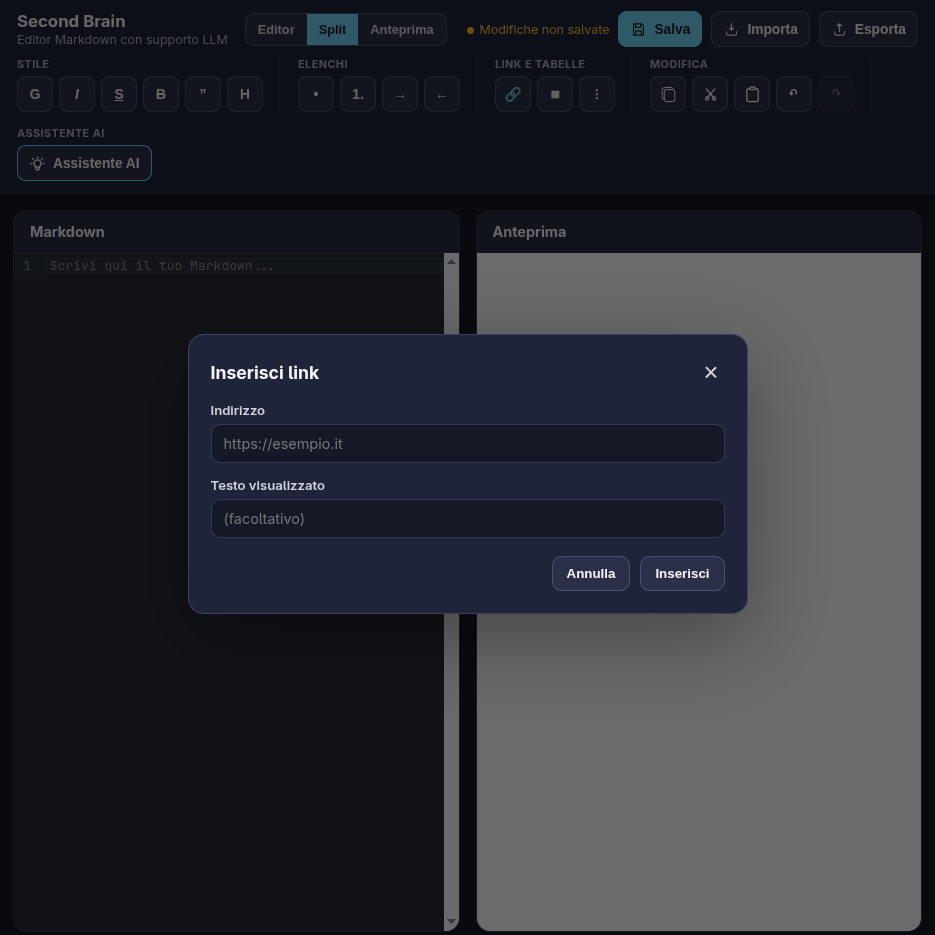
\includegraphics[width=0.6\textwidth]{img/link.png}
    \caption{Finestra di inserimento o modifica di un link}
 \end{figure}

\paragraph{Modifica di un link} Lo stesso bottone "Gestisci link" viene utilizzato anche per la modifica: se, al momento
della pressione,
 il cursore è posizionato sopra o all'interno di un link già presente nel testo (anche senza una vera 
selezione, basta il cursore lampeggiante), la finestra si apre con il titolo "Modifica link" e con i campi "Indirizzo" e 
"Testo visualizzato" già precompilati con i valori correnti: è possibile modificarli e confermare, oppure premere il pulsante 
"Rimuovi link" per eliminare il link mantenendo il solo testo visualizzato come testo normale. Se invece il cursore non si 
trova su alcun link, la finestra si apre vuota in modalità inserimento.

\paragraph{Inserimento di una tabella} Il bottone "Inserisci tabella", quando premuto, apre una nuova finestra con due campi che indicano il numero di righe e di colonne che 
 la nuova tabella dovrà avere.

  \begin{figure}[H]
    \centering
    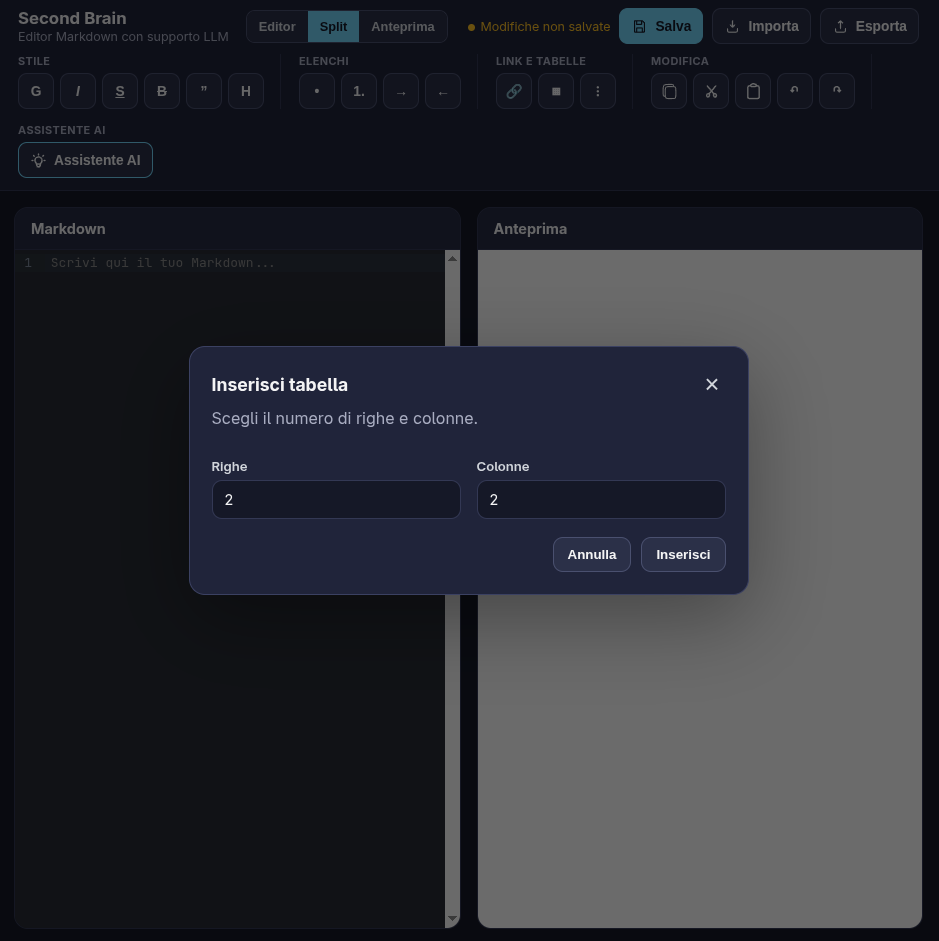
\includegraphics[width=0.6\textwidth]{img/tabella.png}
    \caption{Finestra di inserimento di una tabella}
 \end{figure}

\paragraph{Modifica di una tabella}
Il bottone "Modifica tabella", quando premuto, mostra cinque nuovi bottoni per modificare la tabella selezionata:
aggiungere o rimuovere una riga, aggiungere o rimuovere una colonna, oppure eliminare l'intera tabella.

\subsubsection{Modifica}
La quarta parte è denominata "Modifica" ed è composta da 5 bottoni, che da sinistra a destra sono:
\begin{enumerate}
    \item Copia,
    \item Taglia,
    \item Incolla,
    \item Annulla,
    \item Ripeti.
\end{enumerate}

I primi tre operano sulla porzione di testo selezionata rispettivamente copiandola, tagliandola oppure inserendo nella posizione corrente del cursore il contenuto testuale
precedentemente copiato negli appunti\textsubscript{G} di sistema.
"Annulla" e "Ripeti" permettono, rispettivamente, di annullare l'ultima modifica apportata al documento (Undo\textsubscript{G}) e di 
ripristinare l'ultima modifica annullata (Redo\textsubscript{G}); entrambi i comandi risultano disattivati quando non vi è alcuna
modifica da annullare, o 
da ripristinare.